\begin{frame}{Déclaration vers question}
  Comment transformons-nous les déclarations suivantes en des questions? \\
  \tinygloss{How do we transform the following statements into questions?}
  \begin{columns}
    \column{0.6\textwidth}
      \scriptsize
      \begin{enumerate}
        \item La famille déjeune ensemble le soir.
        \item[$\to$]<2-> \textbf{Est-ce que} la famille déjeune ensemble le soir?
        \item Philippe travaille au bureau le jeudi après-midi.
        \item[$\to$]<4-> \textbf{Est-ce que} Philippe travaille au bureau le jeudi après-midi?
        \item Jacques et ses copains jouent au rugby le mercredi.
        \item[$\to$]<6-> \textbf{Est-ce que} Jacques et ses copains jouent au rugby le mercredi?
        \item Anne parle au téléphone mardi matin.
        \item[$\to$]<8-> \textbf{Est-ce que} Anne parle au téléphone mardi matin?
      \end{enumerate}
    \column{0.4\textwidth}
      \begin{minipage}[c][0.6\textheight]{\linewidth}
        \begin{center}
          \only<-2>{
            \includegraphics[scale=0.5]{déjeuner.png}
          }
          \only<3-4>{
            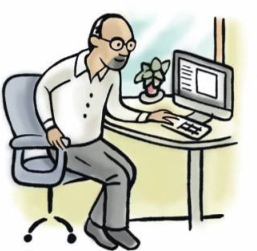
\includegraphics[scale=0.5]{philippe.png}
          }
          \only<5-6>{
            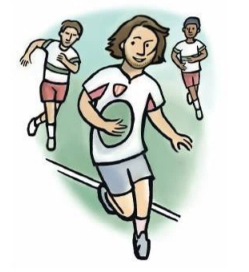
\includegraphics[scale=0.5]{rugby.png}
          }
          \only<7-8>{
            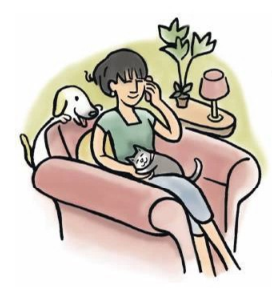
\includegraphics[scale=0.5]{téléphone.png}
          }
        \end{center}
      \end{minipage}
  \end{columns}
\end{frame}